\documentclass[10pt]{beamer}
\usepackage[T1]{fontenc}
\usepackage{mathtools}
\usepackage[french]{babel}
\usepackage{amsmath,amssymb,amsthm}
\usepackage{framed}
\usepackage{lmodern}
\usepackage{utils_slides}
\usepackage{pdfpages}
\usepackage{irif}
\usepackage{listings}
\usepackage{listingsutf8}
\usepackage{tikz}
\usetheme{Madrid}
\definecolor{codegreen}{rgb}{0,0.6,0}
\definecolor{codegray}{rgb}{0.5,0.5,0.5}
\definecolor{codepurple}{rgb}{0.58,0,0.82}
\definecolor{backcolour}{rgb}{0.96,0.96,0.95}
\newcommand*{\pmZpmZ }{p^m\Z \x p^m\Z}
\newcommand*{\ZZpmZ}{\Z^2/\pmZpmZ}
\newcommand*{\ZZnZ}{\Z^2/\nZnZ}
\newcommand{\ZpmZ}{\Z/p^m\Z}
\newcommand{\ZZpm}{\ZpmZ \x \ZpmZ}
\newcommand{\nZnZ}{n\Z \x n\Z}
\newcommand{\Mz}{\Set*{
	\begin{pmatrix}
		p^a  & 0   \\
		j & p^b
	\end{pmatrix}
}{
	\begin{aligned}
		 & (a, b) \in A_0      \\
		 & 0 \le j < p^{b}
	\end{aligned}
}}
\newcommand{\Mk}{\Set*{
	\begin{pmatrix}
		p^a  & 0   \\
		jp^k & p^b
	\end{pmatrix}
}{
	\begin{aligned}
		 & (a, b) \in A_k      \\
		 & 0 \le j < p^{b - k}
	\end{aligned}
}}
\newcommand{\Az}{\Set*{(a,b)}{ a + b \le m}}
\newcommand{\Ak}{\Set*{
	(a,b)}{
	\begin{aligned}
		 & a \le m, b \le m \\
		 & a + b = m + k
	\end{aligned}
}}

\lstdefinestyle{mystyle}{
    breakatwhitespace=false,
    breaklines=true,
    captionpos=b,
    keepspaces=true,
    showspaces=false,
    showstringspaces=false,
    showtabs=false,
	extendedchars=true,
    tabsize=4,
	basicstyle=\ttfamily,
  	mathescape,
	inputencoding=utf8/latin1,
	literate=%
		{é}{{\'e}}{1}%
		{è}{{\`e}}{1}%
		{à}{{\`a}}{1}%
		{ç}{{\c{c}}}{1}%
		{œ}{{\oe}}{1}%
		{ù}{{\`u}}{1}%
		{É}{{\'E}}{1}%
		{È}{{\`E}}{1}%
		{À}{{\`A}}{1}%
		{Ç}{{\c{C}}}{1}%
		{Œ}{{\OE}}{1}%
		{Ê}{{\^E}}{1}%
		{ê}{{\^e}}{1}%
		{î}{{\^i}}{1}%
		{ô}{{\^o}}{1}%
		{û}{{\^u}}{1}%
		{ë}{{\¨{e}}}1
		{û}{{\^{u}}}1
		{â}{{\^{a}}}1
		{Â}{{\^{A}}}1
		{Î}{{\^{I}}}1
}

\lstset{style=mystyle}
\newtheorem{thm}{Theomème}
\newtheorem{pf}{Preuve}
\newtheorem{rmk}{Remarque}
\newtheorem{prp}{Proposition}
\newtheorem{df}{Définition}
\newtheorem{crll}{Corollaire}


\title{Sous-groupes de $\ZZ$}
\subtitle{Projet Mathématiques - Informatique}
\author[Kevin Garnier, Charly Martin Avila, Olivier Brunat]{
	\itshape {Kevin Garnier \\
		Charly Martin Avila}\\
		\vspace*{1cm}
	Dirigé par
	Olivier Brunat
}

\date{Année \the\year}
% Top left and top right  Position of a logo in beamer
\titlegraphic {
\begin{tikzpicture}[overlay,remember picture]
\node[left=0.2cm] at (current page.33){
    
\includegraphics[width=3cm]{logo_upc_big.pdf}
};
\end{tikzpicture}
}

\begin{document}

\begin{frame}
    \titlepage
\end{frame}

\tableofcontents


\section{Quelques simplifications du problème}
\begin{frame}
    \frametitle{Quelques simplifications du problème}
    \tableofcontents[currentsection]
\end{frame}


\subsection{Décomposition de $n$ en éléments irréductibles}
\begin{frame}
    \frametitle{Décomposition de $n$ en éléments irréductibles}
    \begin{block}{Proposition}
        Soit $n = \prod\limits_{i = 1}^k p_i^{\alpha_i}$, avec $p_i$ des nombres premiers, alors
        $$(\ZZ) \isom \prod_{i = 1}^k(\Z/p_i^{\alpha_i}\Z)^2$$
    \end{block}
\end{frame}


\begin{frame}[fragile]
    \frametitle{Décomposition de n en éléments irréductibles}
    \begin{lstlisting}
fonction rho_pollard P n x y k i d
    Si d $\ne$ 1:
        Retourne d
    Sinon :
        x = P(x) mod n
        d = pgcd (| y - x | , n )
        Si i = k :
            Retourne rho_pollard P n x x 2k (i+1) d
        Sinon
            Retourne rho_pollard P n x y k (i+1) d
    \end{lstlisting}
\end{frame}

\subsection{Simplification des sous-groupes}
\begin{frame}
    \frametitle{Simplification des sous-groupes}
    \begin{block}<1->{Proposition}
        $$\Z^2/n\Z \x n\Z \isom \ZZ $$\end{block}
    \begin{block}<2->{Remarque}
        Ainsi le problème se résout à trouver les sous-groupes $G$ de $\Z^2$ tels que
        $$H = \matsqr{a}{c}{b}{d}$$
        et
        $$n\Z \x n\Z \subseteq G = \gen{\vectcolsqr{\bar a}{\bar b}, \vectcolsqr{\bar c}{\bar d}}$$

    \end{block}
\end{frame}


\section{Matrices à coefficients entier et forme normales de Hermite}
\begin{frame}
    \frametitle{Table des matières}
    \tableofcontents[currentsection]
\end{frame}


\subsection{Matrices à coefficients entier}
\begin{frame}
    \frametitle{Matrices à coefficients entier}

    \begin{block}{Proposition}
        Soient $A \in \M_{m,n}(\Z)$ et $Q \in \GL_n(\Z)$, alors
        $$\im AQ = \im A$$
    \end{block}
\end{frame}


\subsection{Formes normales de Hermite}
\begin{frame}
    \frametitle{Formes normales de Hermite}
    \begin{alertblock}{Définition}
        Soit $A \in \M_{m,n}(\Z)$. Alors, il existe une unique matrice échelonnée
        réduite suivant les colonnes $H \in \M_{m,n}(\Z)$ telle qu'il existe $Q \in \GL_n(\Z)$
        avec $H = AQ$. La matrice $H$ s'appelle la forme normale de Hermite de $A$.
    \end{alertblock}
\end{frame}


\section{Génération et énumération des sous-groupes}
\begin{frame}
    \frametitle{Table des matières}
    \tableofcontents[currentsection]
\end{frame}


\subsection{Génération des sous-groupes}
\begin{frame}
    \frametitle{Génération des sous-groupes}
    \begin{itemize}
        \item Dans cette section, nous supposerons que $n$ = ${p}^{m}$
    \end{itemize}
    \begin{alertblock}{Théorème}
        Les seules matrices dont les colonnes génèrent un sous-groupe de $\ZZpmZ$
        sont les matrices de la forme
        $$H =
            \begin{pmatrix}
                p^a & 0   \\
                j   & p^b
            \end{pmatrix}
            \text{avec $a \le m$, $b \le m$ et $j < p^b$}
        $$
        $$ \text{ ou }$$
        $$ H =\begin{pmatrix}
                p^a  & 0   \\
                jp^k & p^b
            \end{pmatrix}
            \text{avec $a \le m$, $b \le m$, $k \le m$ et $j < p^{b - k}$}
        $$
    \end{alertblock}
\end{frame}


\begin{frame}
    \begin{block}{Corollaire}
        Soit la suite $\suit{A}{k}{0 \le k \le n}$ telle que
        \begin{equation*}
            \begin{split}
                &A_0 = \Set*{(a,b)}{ a + b \le m}\\
                &A_k = \Set*{
                    (a,b)}{
                    \begin{aligned}
                         & a \le m, b \le m \\
                         & a + b = m + k
                    \end{aligned}
                }
            \end{split}
        \end{equation*}
        Alors, l'ensemble des matrices du théorème, \cad, les matrices dont les colonnes
        génèrent les sous-groupes de $\ZZpmZ$ est
        $$M = \bigsqcup_{k = 0}^mM_k$$
        où
        \begin{equation*}
            M_k = \Set*{
                \begin{pmatrix}
                    p^a  & 0   \\
                    jp^k & p^b
                \end{pmatrix}
            }{
                \begin{aligned}
                     & (a, b) \in A_k      \\
                     & 0 \le j < p^{b - k}
                \end{aligned}
            }
        \end{equation*}
    \end{block}
\end{frame}


\subsection{Énumération des sous-groupes}
\begin{frame}
    \frametitle{Énumération des sous-groupes}
    \begin{alertblock}{Théorème}
        Soit $\psi: \mathbb{N}^2 \rightarrow \mathbb{N}$ définie par
        Soit
        \app{\psi}{\N^2}{\N}{(p,n)}{\sum_{i=0}^{n}(n-i)p^i + \sum_{i = 0}^{n}\frac{1- p^{n-i+1}}{1 - p}}
        Alors, le nombre de sous groupe de $\ZZpm$ est $\psi(p,m)$
    \end{alertblock}
\end{frame}


\begin{frame}
    \begin{prp}
        Soit $n = \prod\limits_{i = 1}^k p_i^{\alpha_i}$ avec $p_i$ des nombres premiers distincts\\
		Le nombre total de sous-groupes de $\ZZ$ est
		$$\prod_{i = 0}^{k} \psi(p_i,\alpha_i)
			= \prod_i^k\mlarge[3](\sum_{j=0}^{\alpha_i}(\alpha_i-j)p_i^j +%
			\sum_{j = 0}^{\alpha_i}\frac{1- p_i^{\alpha_i-j+1}}{1 - p_i}\mlarge[3])$$
    \end{prp}
\end{frame}


\section{Génération du treillis}
\begin{frame}
    \frametitle{Génération du treillis}
    \tableofcontents[currentsection]
\end{frame}

\begin{frame}[fragile]
    \frametitle{Génération du treillis}
    \begin{lstlisting}
fonction creer_treillis $G$ $T$ =
	$G \leftarrow$ Trier $G$ par la cardinalité
	L = $\NO$
	Pour chaque $u \in G$:
		Pour chaque $v \in  T[u]$:
			Si $\nexists (u,v') \in L$ tel que $v' \subset v $
				Alors $L \cup \set{(u,v)}$
	Retourner $(G,L)$
\end{lstlisting}
\end{frame}


\section{Quelques résultats}
\begin{frame}
    \frametitle{Table des matières}
    \tableofcontents[currentsection]
\end{frame}


\subsection{Pour n = 2}
\begin{frame}
    \frametitle{Pour n = 2}
    \begin{itemize}
        \item Nombre de sous-groupe de $\Z/2\Z \x \Z/2\Z$ : 5
    \end{itemize}
    \begin{figure}
        \centering
        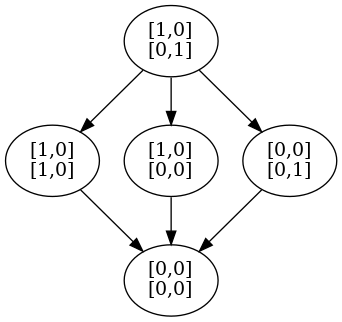
\includegraphics[width=0.5\textwidth]{Z2ZxZ2Z.png}
        \caption{Treillis des sous-groupes de $\Z/2\Z \x \Z/2\Z$ avec les forme normale de Hermite
            correspondantes}
    \end{figure}
\end{frame}


\subsection{Quelques valeur de la suite du nombre de sous-groupes}
\begin{frame}
    \frametitle{Quelques valeur de la suite du nombre de sous-groupes}
    \begin{center}
        \begin{tabular}{|c|c|c|c|c|c|c|c|c|c|c|c|}
            \hline
            n          & 0        & 1 & 2 & 3 & 4  & 5 & 6  & 7  & 8  & 9  & 10 \tabularnewline
            \hline
            $|S(\ZZ)|$ & $\infty$ & 1 & 5 & 6 & 15 & 8 & 30 & 10 & 37 & 23 & 40 \tabularnewline
            \hline
        \end{tabular}
    \end{center}
\end{frame}


\section{Bibliographie}
\begin{frame}
    \frametitle{Table des matières}
    \tableofcontents[currentsection]
\end{frame}


\begin{frame}
    \frametitle{Bibliographie}
    \begin{itemize}
        \item COSTE Michel; \textit{Algèbre linéaire sur les entiers}; Mars 2018
        \item Thomas H. Cormen, Charles Leiserson, Ronald Rivest, Clifford Stein;\\
              \textit{Algorithmique : cours avec 957 exercices et 158 problèmes}, $3^e$ édition, Paris : Dunod; DL 2010
        \item PERNET Clément; \textit{Calcul de formes normales matricielles: de
                  l'algorithmique à la mise en pratique}; Séminaire SIESTE; ENS-Lyon; 12 février 2013
        \item BERHURY Grégory; \textit{Algèbre le grand combat : Cours et exercices};
              $2^e$ édition;
        \item Mario Hampejs, Nicki Holighaus, László Tóth, Christoph Wiesmeyr;\\
              \textit{Representing and counting the subgroups of the group $Z_m \x Z_n$}; 2012
    \end{itemize}
\end{frame}


\end{document}
